This section is a summary of ~\cite[p. 4-7]{BuilAranda20131}. In order to get a
deeper understanding of the SERVICE operator it is mandatory to understand which
problems occur when evaluating the SERVICE operator.
A direct implementation of the SERVICE operator based of the semantics is
infeasible in practice. Given $(\mbox{SERVICE }  x \
P_1)$, if $x$ is not restricted to a finite set, we would have to evaluate $P_1$ over every 
possible SPARQL endpoint in $dom(ep)$. This is obviously impossible. To ensure that $P_1$
only gets evaluated over a finite set of URIs, $x$ needs to be limited to exactly
those. In the W3C standard only indications are provided on how to evaluate the
service operator~\cite{w3standardservice} when the location is a variable and
not an URI. In~\cite{BuilAranda20131} the authors deal with this issue by
providing a notion of boundedness. In order to demonstrate how one could
evaluate a service operator using a variable to evaluate a query over more than
one endpoint the following example is given:
\begin{example}[\cite{BuilAranda20131}]
Let $G$ be an RDF graph that uses triples of the form\\ $(a, service\_address,b)$
with the intention to express that $b$ is a SPARQL endpoint URI with name $a$.
Then we consider the following query $P$ over the graph $G$ in the dataset $DS$:
\begin{align*}
	P=((x, service\_address, y) \AND (\mbox{SERVICE } y \ (z_n,email,z_e)))
\end{align*}
It is easy to see that $P$ is used to compute the list of names and email
addresses that can be retrieved from the SPARQL endpoints stored in the RDF
graph $G$ through the $service\_address$ triple. 
The whole point of this example is to point out that there is a simple practical
way to evaluate $P$ over $G$ that is also feasible:
By evaluating $\ll (x,service\_address,y) \rr^{DS}_G$ first and then for every
mapping $\mu$ in this set we further evaluate $\ll (\mbox{SERVICE } a \ (z_n, email, z_e)
\rr^{DS}_G$, where $a = \mu(y)$. 
\end{example}
Throughout the chapter we will provide four different definitions on how the
destinations of a SERVICE-operator can be bound within a graph pattern if the
destination is a variable. Those definitions were first introduced
in~\cite{BuilAranda20131}.
\begin{enumerate}
	\item Boundedness: Boundedness is a na{\"i}ve semantic approach to the
		problem. After formally defining the property, we will show that
		deciding whether a variable is bound in a graph pattern
		is undecidable and thus not feasible for practical use.

	\item Strong boundedness: Strong boundedness is a syntactical approach to
		the problem. We will, by defining the property provide a recursive
		procedure on how to decide which variables in a graph pattern are
		strongly bound. It will also be shown that if a variable is strongly
		bounded, it is bounded aswell. 
		Although this procedure would be feasible for practical
		use complexity-wise, it is not able to decide whether a graph pattern
		can be evaluated in practice. We will provide an example in form of a
		graph pattern which is feasible to be evaluated in practice but not
		strongly bound.

	\item Service-Boundedness: Service-Boundedness would be the optimal solution for
		deciding which graph patterns can be evaluated in practice. If a pattern
		is service-bounded, it can be evaluated in practice. The problem however
		is, that the definition builds on the definition of boundedness which is
		undecidable. Therefore service-boundedness is not feasible for practical
		use.
	\item Service-Safeness: The definition of Service-Safeness builds on the
		definition of strong boundedness. 
		Service-Safeness is easy to decide and we will show that if a pattern is
		Service-Safe, it is also Service-Bound. This solution should be used in
		practice for the original problem.
\end{enumerate}

In the last section we will discuss the difference of boundedness and strong
boundedness (and thus Service-Boundedness and Service-Safeness because the
latter definitions build on former definitions). 

\section{The four different ways to bind the destination of a SERVICE-operator}

To describe boundedness we need three definitions namely the domain of a graph,
a dataset and a graph pattern.

\begin{definition}[Domain of a graph, a dataset and a graph pattern,\cite{BuilAranda20131}]
    The domain of a graph $G$ denoted $dom(G)$ is defined as $dom(G) = \bigcup\limits_{(u,v,w) \in G}
    vars(u,v,w)$. The domain of a dataset $DS$, denoted $dom(DS)$ is defined as
    $dom(DS) = \bigcup\limits_{G \in names(DS)} dom(G)$.
    The domain of a graph pattern $P$ is denoted $dom(P)$ and refers to the set of URIs that are
mentioned in $P$.
\end{definition}

Boundedness of a variable $x$ in a graph pattern $P$ makes sure that the
variable is always in the domain of every solution $\mu$ and the image $\mu(x)$ is either in the 
domain of the dataset $P$ gets evaluated over, it is a graph name or it is in the domain of the pattern.

\begin{definition}[Boundedness,\cite{BuilAranda20131}]
Let $P$ be a graph pattern and $x \in var(P)$. Then $x$ is bound in $P$ if the
following condition holds:
For every dataset $DS$, every graph $G$ in $DS$ 
and every $\mu \in \ll P \rr^{DS}_G:$\\
\[ x \in dom(\mu) \mbox{ and } \mu(x) \in (dom(DS) \cup names(DS) \cup dom(P)). \]
\end{definition}

Resulting from this definition a very natural way seems to arise to ensure that
a graph pattern $P$ can be evaluated in practice: 
We will now define a na\"ive way to make sure we can evaluate a pattern:
Assuming we want to evaluate a sub-pattern $(\mbox{SERVICE } x \ P_1)$ of $P$
we require $x$ to be bound in $P$. We can then define the problem for deciding if a variable
is bound in a graph pattern $P$:

\begin{framed}\noindent \textbf{BOUND IN PATTERN}\\
	\textbf{INPUT:} A graph pattern $P$ and a variable $x \in var(P)$.\\
	\textbf{QUESTION:} Is $x$ bound in $P$?
\end{framed}
Unfortunately \textbf{BOUND IN PATTERN} is undecidable which can be shown by
reducing from \textbf{SPARQL SAT} to \textbf{BOUND IN PATTERN}.
\begin{framed}\noindent \textbf{SPARQL SAT}\\
	\textbf{INPUT:} A graph pattern $P$.\\
	\textbf{QUESTION:} Does a dataset $DS$ and a graph $G$ in $DS$ exist such
	that $\ll P \rr^{DS}_G$?
\end{framed}
It is a well known result that $\textbf{SPARQL SAT}$ is undecidable~\cite{angles2008expressive}.

\begin{theorem}[\cite{BuilAranda20131}]
	\textbf{BOUND IN PATTERN} is undecidable.
\end{theorem}
\begin{proof}
By providing a reduction from the \textbf{SPARQL SAT} problem to the
\textbf{VARIABLE BOUND IN PATTERN} Problem we will be able to prove the theorem.
Let $P$ be a graph pattern, i.e., an arbitrary instance of \textbf{SPARQL SAT} and
$x,y,z$ variables not mentioned in $P$. Then define the graph pattern $Q$,
i.e. the instance of \textbf{VARIABLE BOUND IN GRAPH} pattern as follows: $Q =
((x,y,z) \UNION  P)$ and choose $x$ to be the potentially bound variable.
It remains to show that $x$ is bound in $Q$  if and only if $P$ is not
satisfiable.\\
$(\Rightarrow)$:\\
Assume now that the variable $x$ is bound in $Q$, i.e., for every RDF graph $G$
in $DS$ and every $\mu \in \ll Q \rr^{DS}_G:$ $x \in dom(\mu)$ and $\mu(x) \in
(dom(DS) \cup names(DS) \cup dom(P))$. Let $DS$ be an arbitrary dataset and let
$G$ be an arbitrary graph in $DS$.
\begin{enumerate}
	\item $\ll Q \rr^{DS}_G = \emptyset$. Because of $\ll Q \rr^{DS}_G =
		\emptyset$, we can instantly see that $P$ is unsatisfiable.
	\item $\ll Q \rr^{DS}_G \neq \emptyset$.\\
		Let $\mu \in \ll Q \rr^{DS}_G$ be arbitrary.
		We can instantly see that $x \in dom(\mu)$ must hold. 
		Because by construction $P$ doesn't contain $x$, 
		$\mu \notin \ll P \rr^{DS}_G$. Thus $P$ is unsatisfiable.
\end{enumerate}
\noindent$(\Leftarrow)$:\\
Assume now that $P$ is not satisfiable. Let $DS$ be an arbitrary dataset and let
$G$ be an arbitrary graph in $DS$. Because of our initial assumption $\ll P
\rr^{DS}_G = \emptyset$. We will now further distinguish between two cases:
\begin{enumerate}
	\item $\ll Q \rr^{DS}_G = \emptyset$. Then $x$ is trivially bound in $Q$.
	
	\item $\ll Q \rr^{DS}_G \neq \emptyset$.\\
		Let $\mu \in \ll Q \rr^{DS}_G$ be arbitrary.
		We can instantly see by construction of $Q$ that $x \in
		dom(\mu)$ must hold. By SPARQL semantics $\mu(x) \in dom(DS)$. Thus $x$
		is bound in $Q$.\qedhere
\end{enumerate}
\end{proof} 

As deciding boundedness for a variable is undecidable the notion of
\emph{strong boundedness} is introduced, which is a syntactic condition and
efficiently verifiable. 

\begin{definition}[Strong
	Boundedness~\cite{BuilAranda20131}]\label{def:strongboundedness}
Let $P$ be a graph pattern. Then the set of strongly bound variables in $P$,
denoted by $SB(P)$, is recursively defined as follows.

\begin{itemize}
\item if $P =t$, where $t$ is a triple pattern, then $SB(P) = vars(t)$;
\item if $P = (P_1 \ AND \ P_2)$, then $SB(P) = SB(P_1) \cup SB(P_2)$ 
\item if $P = (P_1  \ UNION \ P_2)$, then $SB(P) = SB(P_1) \cap SB(P_2)$ 
\item if $P = (P_1 \ OPT \ P_2)$, then $SB(P) = SB(P_1)$ 
\item if $P = (GRAPH \ u \ P_1)$, with $u \in U\cup V$, 
then\\
\begin{align*}
	SB(P) = 
\begin{cases} 
    \emptyset & \mbox{$u \in U$} \\
    SB(P_1) \cup u &\mbox{$u \in V$} 
\end{cases}
\end{align*}

\item if $P = (SERVICE \ u \ P_1)$, with $u \in U \cup V$, then $SB(P) = \emptyset$.
\end{itemize}
\end{definition}

It is a simple observation that this recursive definition collects a set of
variables that are guaranteed to be bound in $P$. The following proposition
documents this observation.

\begin{proposition}[\cite{BuilAranda20131}]\label{sbinb}
For every graph pattern $P$ and a variable $x \in var(P)$, if $x \in SB(P)$,
then $x$ is bound in $P$.
\end{proposition}
The proof is a very straight forward induction and can be found
in~\cite[Appendix A]{BuilAranda20131}.

We notice that this proposition is not an if and only if statement and hence we may be
able to provide a pattern $P$ where variables $x \in vars(P)$ exist, which are bound but not
strongly bound. Furthermore another example is provided which makes things more
complicated. In Example~\ref{ex:boundedbad} we provide a graph pattern $P$ where a variable in the
destination of a SERVICE-operator occurs which is neither bounded nor strongly
bounded. We will then provide a plan on how to evaluate $P$ and thus show that
the definition of neither boundedness nor strongly boundedness is sufficient for
practical usage. 

\begin{example}\label{ex:boundedbad}
Consider the following graph pattern:
\begin{align*}
P_1 = [(x,service\_description,z) \UNION ((x,service\_address, y) \AND
\\\
(\mbox{SERVICE } y \ (x_n,email,x_e)))]
\end{align*}
The variables $x$ and $z$ store the name of a SPARQL endpoint and a description of its
functionalities through the $service\_description$ triple. The variables $x$ and $y$ store the
name of a SPARQL endpoint and the URI where it is located through the
service\_address triple. The problem is, that variable $y$ is neither bound nor
strongly bound in $P_1$. However we can still easily evaluate the pattern by
assuming a dataset $DS$ and an RDF graph $G$ in $DS$:\\
Compute $\ll (x, service\_description,z)\rr^{DS}_G$, then compute \\
$\ll (x, service\_addres,y) \rr^{DS}_G$ and finally for every
$\mu \in \ll (x, service\_addres,y) \rr^{DS}_G$, compute $\ll (\mbox{SERVICE }
a \ (x_n,email,x_e))\rr^{DS}_G$ with $a = \mu(y)$. We can easily see that $y$ is
bound and strongly bound in the subpattern \\ $((x,service\_address, y) \AND
(\mbox{SERVICE } y \ (x_n,email,x_e)))$ of $P_1$ and thus the evaluation is possible.
\end{example}

\noindent To describe a condition that ensures all SPARQL queries containing the SERVICE
operator can be evaluated in practice, the definition of Service-Boundedness is
introduced. The definition of service-boundedness uses a parse tree to make sure
that our evaluation takes bounded subpatterns into account.

\begin{example}\label{ex:parsetree}[\cite{BuilAranda20131}]
Parse tree $\T(Q)$ for the graph pattern \\ $Q = ((y,a,z) \UNION ((x,b,c) \AND (\mbox{SERVICE } x \ (y,a,z))))$.

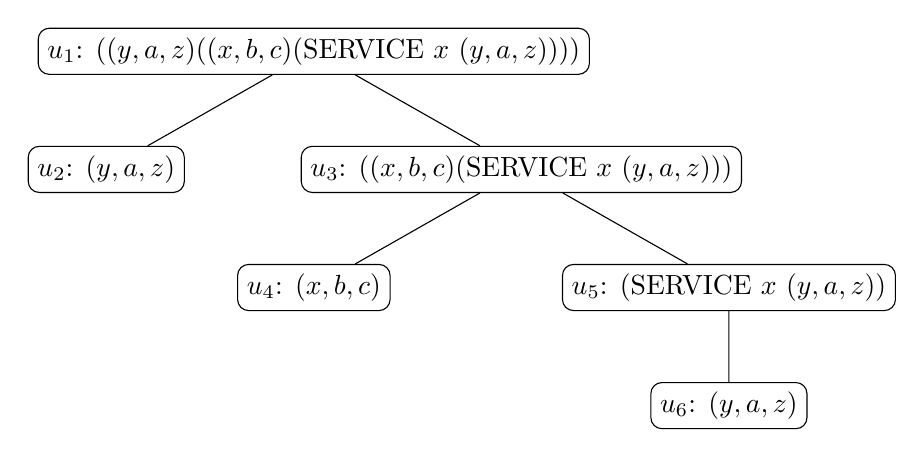
\begin{tikzpicture}[sibling distance=15em,
  every node/.style = {shape=rectangle, rounded corners,
    draw, align=center, top color=white}]]
  \node {$u_1$: $((y,a,z) \UNION ((x,b,c) \AND (\mbox{SERVICE } x \ (y,a,z))))$}
    child { node {$u_2$: $(y,a,z)$} }
    child { node {$u_3$: $((x,b,c) \AND (\mbox{SERVICE } x \ (y,a,z)))$}
      child { node {$u_4$: $(x,b,c)$}}
      child { node {$u_5$: $(\mbox{SERVICE } x \ (y,a,z))$}
	  child	{ node {$u_6$: $(y,a,z)$}} }};
\end{tikzpicture}

\end{example}

\begin{definition}[Parse Tree, \cite{BuilAranda20131}]
	A parse tree of a graph pattern $P$, $\T(P)$ is a tree where each
	node is a sub-pattern of $P$. Each node has an identifier.
	In the parse tree the child relation is used to store the structure of the
	sub-patterns of the graph pattern. The root of the parse tree contains the pattern $P$. Then, 
	in the child(ren) of $P$ the pattern is split up into the respective sub-pattern(s). This is done recursively 	until a node contains only a triple. 
%Assume we have a SPARQL pattern $P$. 
%	We will construct the parse tree $(V,E,r,\lambda)$, where $V$ is the set of vertices, 
%	$E$ the set of edges, $r$ the root and $\lambda$ a labelling function as follows:
	
	
\end{definition}
In Example~\ref{ex:parsetree} a parse tree can be found


Using the definition of a Parse Tree, Service-Boundedness can be defined.

\begin{definition}[\cite{BuilAranda20131}]
	A graph pattern $P$ is service-bound if for every node $u$ of $\T(P)$ with
	label $(SERVICE \ x\  P_1)$, it holds that
	\begin{enumerate}
		\item there exists a node $v$ of $\T(P)$ with label $P_2$ such that $v$
			is an ancestor of $u$ in $\T(P)$ and $x$ is bound in $P_2$,
		\item $P_1$ is service-bound.
	\end{enumerate}
\end{definition}

Corresponding to this definition we will introduce the \textbf{SERVICE BOUND}
problem:
\begin{framed}\noindent \textbf{SERVICE BOUND}\\
	\textbf{INPUT:} A graph pattern $P$.\\
	\textbf{QUESTION:} Is $P$ service-bound?
\end{framed}

Intuitively one can already imagine that deciding the \textbf{SERVICE BOUND}
problem is undecidable because it uses boundedness in it.

\begin{theorem}[\cite{BuilAranda20131}]
	\textbf{SERVICE BOUND} is undecidable.
\end{theorem}
\begin{proof}
By providing a reduction from the \textbf{SPARQL SAT} problem to the  
\textbf{SERVICE BOUND} problem we will be able to show undecidability.
Let $P$ be a graph pattern, i.e., an arbitrary instance of \textbf{SPARQL SAT} and
$x,y,z,x',y',z'$ variables not mentioned in $P$.
Also assume that $P$ does not mention the operator SERVICE which is not required
to make the SPARQL satisfiability problem undecidable.
Then define the graph pattern $Q$, i.e., the instance of \textbf{SERVICE BOUND} as: 
\begin{align*}
	Q = (((x,y,z) \UNION  P) \AND (\mbox{SERVICE } x \ (x', y', z'))).
\end{align*}

\noindent It remains to show that $Q$ is service-bound if and only if $P$ is not
satisfiable.

\bigskip\noindent
$(\Leftarrow)$ \quad If $P$ is not satisfiable, then $Q$ is equivalent to the
pattern: 
\begin{align*}
	Q' = ((x,y,z)) \AND (\mbox{SERVICE} \ x \ (x', y', z')).
\end{align*} 
But $Q'$ is service bound because $x$ is bound in $Q'$: Assume an
arbitrary dataset $DS$, let $G$ be in $DS$. Then 
for any $\mu \in \ll Q' \rr^{DS}_G$, $x \in dom(\mu)$ and for sure $\mu(x) \in
(dom(DS) \cup names(DS) \cup dom(P))$ by semantics of SPARQL and the fact that
$x$ occurs in the triple pattern $(x,y,z)$.


\bigskip\noindent
$(\Rightarrow)$\quad Assume that $P$ is satisfiable. Then we know that variable
$x \not\in vars(P)$ and thus we have that $x$ is not a bound variable in $Q$,
and thus because $x$ occurs in a service operator, $Q$ is not service bound.
\end{proof}

As the problem of undecidability prevails with the definition of
Service-Boundedness, we can again use the syntactic condition, i.e., strong boundedness to define
Service-Safeness which is the same as service-boundedness but uses strongly
boundedness instead of boundedness. We know from
Definition~\ref{def:strongboundedness} that evaluating if a variable is strongly
bound in a graph pattern can be done efficiently.

\begin{definition}[Service Safeness~\cite{BuilAranda20131}]
	A graph pattern $P$ is service-safe if for every node $u$ of $\T(P)$ with
	label $(SERVICE \ x \ P_1)$ it holds that:
	\begin{enumerate}
		\item there exists a node $v$ of $\T(P)$ with label $P_2$ such that $v$
			is an ancestor of $u$ in $\T(P)$ and $x \in SB(P_2)$.
		\item $P_1$ is service safe.
	\end{enumerate}
\end{definition}

As corollary to Proposition 1, the following proposition is obtained:
\begin{proposition}[\cite{BuilAranda20131}]
	If a graph pattern $P$ is service-safe, then $P$ is service-bound.
\end{proposition}

\section{The difference between boundedness and strong boundedness}
It remains to find out what is the difference between strong boundedness
and boundedness. Because boundedness is not equivalent to strong-boundedness, there
must be patterns which are bounded but not strongly bounded. The following problem could arise:
Assume a pattern is bounded but not strongly bounded. Then it is feasible to be evaluated, 
but the proposed algorithm returns that it is not.

\begin{example}\label{bbutnotsbound}
	\begin{align*}
		P = (x,a, b) \OPT (x, a, y).
	\end{align*}
	$y$ is bound in $P$ because for every RDF graph $G$ in $DS$ and
	every $\mu \in \ll P \rr^{DS}_G$ we have that $y \in dom(\mu)$ and
	$\mu(y) \in (dom(DS))$: Assume we have a $\mu \in \ll P \rr^{DS}_G$. Then $x
	\in dom(\mu)$ by semantics of OPT. Assume w.l.o.g. $\mu(x) = c$. Then
	$(c,a, b) \in G$. But then the mapping $\{ x \mapsto c , y\mapsto b \}
	\in \ll P \rr^{DS}_G$.
	The set of strongly bound variables contains
	only $x$, i.e., $SB = \{ x \}$ by Definition~\ref{def:strongboundedness}.
\end{example}

Example~\ref{bbutnotsbound} shows that there patterns 
which are bound but not strongly bound. Inpired by Example~\ref{bbutnotsbound}
we can establish the following result.
%Consider now service safeness, boundness and the following pattern:
%\begin{align*}
%	P = (((x,a, b) \ OPT \ (x, a, y)) \  AND \ (SERVICE \ y \  (a,b,w)))
%\end{align*}
%Pattern $P$ is service-bound but not service-safe. It is obviously possible to
%evaluate $P$. Looking at these examples and noticing that $P$ is contained in
%the query 
%\begin{align*}
%	Q = ((x,a, y) \  AND \ (SERVICE \ y \ (a,b,w)))
%\end{align*} which is obviously service-safe, one could propose that for every
%service-bound query, there is a service-safe query where the service-bound query
%is contained in the service-safe query and also the other way round. For our
%examples this would mean $P \equiv Q$, where $P$ is service-bound but not
%service-safe and $Q$ is service-bound and service-safe.

\begin{theorem}\label{ezprop}
	The problem of verifying, given a graph pattern $P$ in a SPARQL fragment
	$\mathbf{P}$ and a variable $x \in
	var(P)$, whether $x$ is bound in $P$ is as hard as deciding $(P_1 \AND 
	P_2)
	\equiv (P_1 \OPT P_2)$ %for every subpattern $(P_1 \OPT  P_2)$ of $P$% 
	in the SPARQL fragment $\mathbf{P}$.
\end{theorem}
\begin{proof}
	It is very easy to decide strong boundedness and Proposition~\ref{sbinb}
	shows that if a variable $x$ is in $SB(P)$ then $x$ is also bounded in $P$.
	We thus modify our pattern $P$ in such a way, that $SB(P)$ collects all the
	variables which are bounded, even those which are only bounded but not strongly
	bounded.
	Assume $x$ is bounded in $P$ and $x \notin SB(P)$.
	There must thus be a subpattern $Q$ where $x \in vars(Q)$ but $x \notin
	SB(Q)$. We will thus go through every step of the recursive approach of
	Definition~\ref{def:strongboundedness} to find the culprit subpattern.
	\begin{itemize}
		\item If $Q$ is a triple $t$ then $SB(Q) = var(t)$ and by assumption
			that $x \in vars(Q)$ we get that $x \in SB(Q)$. 

		\item If $Q$ is $(P_1 \AND P_2)$ then $SB(Q) = SB(P_1) \cup SB(P_2)$. By
			assumption we know that $x \in vars(Q)$. By semantics of $\cup$ we
			get that $x \in SB(Q)$. 
			
		\item If Q is $(P_1 \UNION  P_2)$ then $SB(P) = SB(P_1) \cap SB(P_2)$.
			By assumption we have that $x \in vars(P_1 \UNION P_2)$.
			Assume $x \notin SB(Q)$. 
			We have a case distinction:
			\begin{enumerate}
				\item $x \in SB(P_1)$ and $x \in SB(P_2)$.
				 We instantly see by semantics of $\cap$ that $x \in SB(Q)$. 

				\item Assume w.l.o.g. that $x \in SB(P_1)$ but $x \notin SB(P_2)$. 
					This contradicts the fact that $x$ is bounded in $P$:
					We could construct a dataset $DS$ with a graph $G$ in it s.t. there
					is a solution $\mu \in \ll P_2
					\rr^{DS}_G$. By assumption we would then have that $x \notin dom(\mu)$.
			\end{enumerate}

		\item If $Q$ is $(P_1 \OPT  P_2)$ we have by definition of SB that $SB(P) = SB(P_1)$
			So a variable $x$ gets lost if it is in $SB(P_2)$, but not in
			$SB(P_1)$. When we have the case that $x$ is bound in $Q$ but not
			strongly bounded in $Q$ we must thus have $(P_1 \AND  P_2) \equiv
			(P_1 \OPT  P_2)$ for every DS, Graph and $\mu \in \ll Q
			\rr^{DS}_G$.

		\item If $Q$ is $(\mbox{GRAPH } u \ P_1)$. We have a case distinction:
			\begin{enumerate}
				\item If $u \in \V$ then it is obvious that if $x \in vars(Q)$ then 
					$x \in SB(Q)$ holds because $vars(Q) = SB(Q)$.
				\item If $u \in \U$ no variables in $vars(Q)$ are bounded because we could
					assume a dataset $DS$ with a graph $G$ in it. Assume
					further that $u \notin names(DS)$. Then $\ll Q \rr^{DS}_{G}
					= \emptyset$. Then assume $P = Q \AND (x',y,z)$. 
					We can easily see that $\ll P \rr^{DS}_{G} \neq \emptyset$.
					But then there is a mapping $\mu \in \ll P \rr^{DS}_{G}$
					but $x \notin dom(\mu)$ and thus $x$ would not be bound in $P$.
			\end{enumerate}

		\item If $Q = (\mbox{SERVICE }  u \ P_1)$ We have a case distinction:
			\begin{enumerate}
				\item If $u \in \V$. We again have two cases. 
					\begin{enumerate}
						\item $u = x$. 
							Assume a dataset $DS$ with a graph $G$ in it.	
							Assume $\mu \in \ll P\rr^{DS}_G$ arbitrary.
							Then $x$ is not bound in $P$ because $\mu(x) \notin (dom(DS) \cup
							names(DS) \cup dom(P))$ could hold because there
							might be an URI referring to an endpoint which is
							not in $(dom(DS) \cup
							names(DS) \cup dom(P))$.
						\item $x \in SB(P_1)$ But then we could possibly have that
							$\mu(x) \notin (dom(DS) \cup names(DS) \cup dom(P))$
					\end{enumerate}

				\item If $u \in \U$ no variables in $vars(Q)$ are bounded because we
					don't know whether $u \in dom(ep)$, SERVICE returns the empty
					mapping $\mu_\emptyset$ in this case by SPARQL semantics. Thus if $x \in vars(Q)$,
					$x \notin SB(Q)$ but $x$ is not bounded in $P$ either
					because $x \notin \mu_\emptyset$.
			\end{enumerate}
	\end{itemize}

	To modify our pattern $P$ in such a way, that $SB(P)$ collects all the
	variables which are bound we would need to replace all occurrences of  $(P_1
	\OPT P_2)$ with $(P_1 \AND P_2$ iff $(P_1 \AND  P_2) \equiv	(P_1 \OPT  P_2)$
	holds.
\end{proof}

Note that deciding $(P_1 \AND P_2) \equiv
(P_1 \OPT  P_2)$ is undecidable for general SPARQL patterns and is the reason
why deciding \textbf{BOUND IN PATTERN} is undecidable. Furthermore it is the key to explain
the difference between strongly boundedness and boundedness.

\begin{corollary}
	The problem of verifying, given a graph pattern $P$ in a fragment
	$\mathbf{P}$ , whether $P$ is
	service-bound is as hard as deciding $(P_1 \AND \ P_2) \equiv (P_1 \OPT
	P_2)$ for every subpattern $(P_1 \OPT P_2)$ of $P$ in the fragment
	$\mathbf{P}$.
\end{corollary}

\begin{proof}
	It is obvious that checking the boundedness in the ancestor of a service
	node causes the undecidability. Thus we use the result in Theorem~\ref{ezprop} to
	show that deciding whether a variable $x$ is bound in this ancestor is as
	hard as deciding $(P_1 \AND P_2)
	\equiv (P_1 \OPT  P_2)$ for every subpattern $(P_1 \OPT P_2)$ of $P$, where
	$P$ is the label of the ancestor node.
\end{proof}
%\begin{corollary}
%	The problem of verifying, given a well-designed graph pattern $P$, whether $P$ is
%	service-bound is NP-hard.
%\end{corollary}
%\begin{proof}
%	Hier sind auch meine results wichtig weil $P_1$ und $P_2$ wiederum SERVICE
%	und GRAPH beinhalten koennten. Sonst ist natuerlich
%	$\cite{pichler2014containment}$ zu zitieren.
%\end{proof}


